\documentclass[11pt,a4paper]{article}

\usepackage[T1]{fontenc}
\usepackage[utf8]{inputenc}
\usepackage[margin=2.1cm]{geometry}
\usepackage{amsmath,amssymb}
\usepackage{xcolor}
\usepackage{listings}
\usepackage{enumitem}
\usepackage{booktabs}
\usepackage{tikz}
\usetikzlibrary{positioning,arrows.meta,shapes.geometric,fit,backgrounds,calc}
\usepackage[hidelinks]{hyperref}

\definecolor{codebg}{gray}{0.96}
\definecolor{kw}{RGB}{0,90,160}
\lstset{
  basicstyle=\ttfamily\small,
  keywordstyle=\color{kw}\bfseries,
  commentstyle=\color{gray},
  columns=fullflexible,
  keepspaces=true,
  breaklines=true,
  language=Python,
  showstringspaces=false,
  backgroundcolor=\color{codebg},
  frame=none,
}
\newcommand{\code}[1]{\texttt{\detokenize{#1}}}
\newcommand{\fn}[2]{%
  \par\smallskip\noindent\texttt{\detokenize{#1}}\\[1pt]%
  \nopagebreak\hspace*{1.2em}\begin{minipage}[t]{0.93\linewidth}\small #2\end{minipage}\par
}

\title{\textbf{Genetic Fuzzy Tree (GFT) for N-CMAPSS}\\[2pt]
\large Code documentation\\[4pt]
\normalsize \texttt{gft.py} \textperiodcentered\ \texttt{datasets.py} \textperiodcentered\
\texttt{leaf\_search.py} \textperiodcentered\ \texttt{ncmapss\_features.py} \textperiodcentered\
\texttt{gft\_analysis.py} \textperiodcentered\ \texttt{run.py}}
\author{}
\date{}

\begin{document}
\maketitle
\vspace{-2.4em}

\section{Overview}

The model is a \emph{nested} Genetic Fuzzy Tree trained \textbf{end-to-end} by a
real-coded genetic algorithm. It is a genuine tree, not a chain of independent
stages: small sub-FIS are composed, and the \emph{output of a child FIS is an input
of its parent}.

\begin{itemize}[leftmargin=1.4em,itemsep=1pt]
\item \textbf{Leaves --- diagnosis.} One FIS per health modifier maps residualised
      cruise sensors to an estimated health parameter, \code{[sensors] -> theta_hat}.
      Leaves are \emph{supervised}: each has a $\theta$ target.
\item \textbf{Spool nodes --- aggregation.} \code{hp} and \code{lp} fuse leaf outputs
      into one \emph{latent} shaft-damage value in $[0,1]$. No target of their own.
\item \textbf{Root --- prognosis.} \code{RUL(hp, lp)} outputs remaining useful life.
\end{itemize}

\noindent The whole genome is optimised against a single scalar loss; the latent
spool values are discovered by the GA.

\paragraph{The claim being defended.} The purpose is \emph{not} to beat a recurrent
network on RMSE. It is to obtain a prognostic model whose intermediate nodes are
physically named and readable, and which generalises to \textbf{unseen failure modes}
better than a lifetime prior. Every design decision below is subordinate to that, and
several trade accuracy for it deliberately.

\paragraph{Fuzzy model.} Each FIS is a \textbf{zero-order Takagi--Sugeno} system on a
\emph{full grid} of rules. Inputs are fuzzified with a \textbf{Ruspini partition}
(triangles summing to 1 everywhere). With the product t-norm and the full grid, the
firing strengths sum to exactly~1,
\[
  \sum_{\text{rules}}\ \prod_d \mu_{d,i_d}(x_d)
  \;=\; \prod_d \Big(\sum_i \mu_{d,i}(x_d)\Big) \;=\; 1 ,
\]
so the Sugeno weighted average collapses to a dot product with the rule singletons:
\[
  y(x)\;=\;\sum_r f_r(x)\, c_r .
\]

\paragraph{The genome holds \emph{both} halves of the fuzzy system.} A genetic fuzzy
system that tunes only the consequents is half a GFS. Here the genome carries the
\textbf{antecedents} (where the membership functions sit, \S\ref{sec:mf}) and the
\textbf{consequents} (one singleton per rule, \S\ref{sec:mono}).

\paragraph{The tree must beat one line of arithmetic.} Every result is reported next
to
\[
  \widehat{\mathrm{RUL}} \;=\; c-\mathrm{age},
  \qquad c=\text{one fitted constant},
\]
which uses \emph{zero sensors}. On units with similar lifetimes this baseline is
strong, and a GA given \code{age} at the root will reproduce it while the leaves
become decoration. Hence \S\ref{sec:eval}.

\section{Tree architecture}

\begin{center}
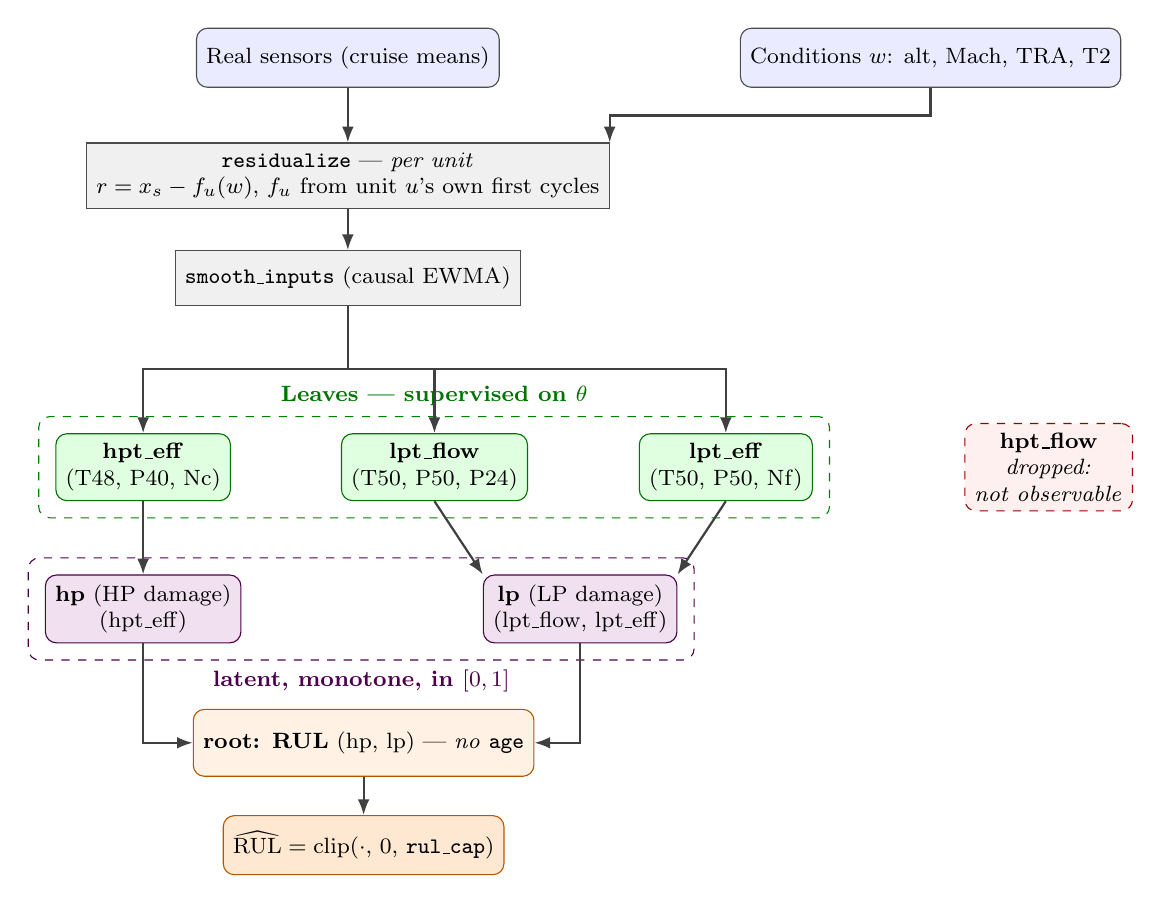
\begin{tikzpicture}[
  io/.style={rectangle, rounded corners, draw=black!70, fill=blue!8,
             align=center, inner sep=3.5pt, font=\footnotesize, minimum height=0.75cm},
  proc/.style={rectangle, draw=black!70, fill=gray!12,
             align=center, inner sep=3.5pt, font=\footnotesize, minimum height=0.7cm},
  fis/.style={rectangle, rounded corners, draw=green!45!black, fill=green!12,
             align=center, inner sep=3.5pt, font=\footnotesize, minimum height=0.85cm},
  spool/.style={rectangle, rounded corners, draw=violet!60!black, fill=violet!12,
             align=center, inner sep=3.5pt, font=\footnotesize, minimum height=0.8cm},
  outb/.style={rectangle, rounded corners, draw=orange!70!black, fill=orange!18,
             align=center, inner sep=3.5pt, font=\footnotesize, minimum height=0.75cm},
  dead/.style={rectangle, rounded corners, draw=red!60!black, dashed, fill=red!6,
             align=center, inner sep=3.5pt, font=\footnotesize, minimum height=0.85cm},
  arr/.style={-{Latex[length=2mm]}, thick, black!75},
  darr/.style={-{Latex[length=2mm]}, thick, dashed, black!55},
]

\node[io]   (sens)   at (0,0)      {Real sensors (cruise means)};
\node[io]   (w)      at (7.4,0)    {Conditions $w$: alt, Mach, TRA, T2};
\node[proc] (resid)  at (0,-1.5)   {\texttt{residualize} --- \emph{per unit}\\ $r=x_s-f_u(w)$, $f_u$ from unit $u$'s own first cycles};
\node[proc] (smooth) at (0,-2.8)   {\texttt{smooth\_inputs} (causal EWMA)};

\node[fis]  (f1) at (-2.6,-5.2) {\textbf{hpt\_eff}\\ (T48, P40, Nc)};
\node[fis]  (f2) at ( 1.1,-5.2) {\textbf{lpt\_flow}\\ (T50, P50, P24)};
\node[fis]  (f3) at ( 4.8,-5.2) {\textbf{lpt\_eff}\\ (T50, P50, Nf)};
\node[dead] (f4) at ( 8.9,-5.2) {\textbf{hpt\_flow}\\ \emph{dropped:}\\ \emph{not observable}};

\node[spool] (hp) at (-2.6,-7.0) {\textbf{hp}\ (HP damage)\\ (hpt\_eff)};
\node[spool] (lp) at ( 2.95,-7.0) {\textbf{lp}\ (LP damage)\\ (lpt\_flow, lpt\_eff)};

\node[fis, draw=orange!70!black, fill=orange!10] (rul) at (0.2,-8.7)
  {\textbf{root: RUL}\ (hp, lp)\ ---\ \emph{no} \texttt{age}};
\node[outb] (out) at (0.2,-10.0) {$\widehat{\mathrm{RUL}}=\mathrm{clip}(\cdot,\,0,\,\texttt{rul\_cap})$};

\draw[arr] (sens) -- (resid);
\draw[arr] (w.south) -- ++(0,-0.35) -| (resid.north east);
\draw[arr] (resid) -- (smooth);
\draw[arr] (smooth.south) -- ++(0,-0.8) -| (f1.north);
\draw[arr] (smooth.south) -- ++(0,-0.8) -| (f2.north);
\draw[arr] (smooth.south) -- ++(0,-0.8) -| (f3.north);
\draw[arr] (f1.south) -- (hp.north);
\draw[arr] (f2.south) -- (lp.north west);
\draw[arr] (f3.south) -- (lp.north east);
\draw[arr] (hp.south) |- (rul.west);
\draw[arr] (lp.south) |- (rul.east);
\draw[arr] (rul) -- (out);

\begin{scope}[on background layer]
  \node[draw=green!50!black, dashed, rounded corners, inner sep=6pt,
        fit=(f1)(f2)(f3),
        label={[green!45!black,font=\footnotesize\bfseries]above:{Leaves --- supervised on $\theta$}}] {};
  \node[draw=violet!60!black, dashed, rounded corners, inner sep=6pt,
        fit=(hp)(lp),
        label={[violet!60!black,font=\footnotesize\bfseries]below:{latent, monotone, in $[0,1]$}}] {};
\end{scope}
\end{tikzpicture}
\end{center}

\noindent Each engine's sensors are stripped of \emph{its own} new-condition
signature (\S\ref{sec:prep}), EWMA-smoothed along cycles, then fed to the leaves.
\code{hp} is a \textbf{single-input node}: a monotone 1-D calibration from HPT
efficiency modifier to HP-shaft damage. That is intentional --- see
\S\ref{sec:leafsearch}. A one-input FIS is still a legitimate, readable fuzzy node,
and \code{plot_surface_node} renders it as a curve.

\paragraph{Three tree variants} live in \code{gft.py}:

\begin{center}
\begin{tabular}{llp{8.1cm}}
\toprule
\textbf{constant} & \textbf{params} & \textbf{role} \\
\midrule
\code{TREE}     & 158 & default \\
\code{TREE_LP1} & 109 & drops the coupled \code{lpt_eff}; fully spool-specific \\
\code{TREE_AGE} & 180 & ablation control --- restores \code{age} at the root \\
\bottomrule
\end{tabular}
\end{center}

\paragraph{Editing the topology.} A tree is a list of
\code{(name, [inputs], theta_target_or_None)}. An input is a data column (sensor or
\code{"age"}) or the name of an earlier node. Children must precede parents, the root
must be named \code{"RUL"}, and a node takes at most 3 inputs. Per-input membership
counts are given by writing an input as a pair:

\begin{lstlisting}
_LEAVES = [
    ("hpt_eff",  [("T48", 5), "P40", "Nc"], "HPT_eff_mod"),  # T48 -> 5 fuzzy sets
    ("lpt_flow", ["T50", "P50", "P24"],     "LPT_flow_mod"),
    ("lpt_eff",  ["T50", "P50", "Nf"],      "LPT_eff_mod"),
    ("hp", ["hpt_eff"],             None),   # single-input spool node
    ("lp", ["lpt_flow", "lpt_eff"], None),
]
TREE = _LEAVES + [("RUL", ["hp", "lp"], None)]
\end{lstlisting}

\noindent A node's rule count is the \emph{product} of its inputs' set counts, so
$(5,3,3)\Rightarrow45$ rules and 45 consequent genes for that node alone.

\section{Learnable membership functions}\label{sec:mf}

\paragraph{Why quantile centres fail.} Fixing the antecedent centres at data
quantiles is pathological for a health modifier: $\theta\approx0$ for most of a
unit's life and only plunges at the end, so the \emph{median} sits at $\approx0$.
With $k=3$, two of three centres collapse into the healthy plateau and the entire
degraded regime --- the only part that matters --- is described by one triangle's
ramp. It is calibrating an EGT gauge with tick marks at $0^\circ$, $1^\circ$ and
$900^\circ$C.

\paragraph{Centres \emph{are} the membership functions.} Under a Ruspini partition
the fuzzy sets of one variable are entirely determined by their ordered centres
$c_1<\dots<c_k$. So the GA evolves them.

\paragraph{Encoding: gaps, not positions.} A GA mutating positions directly would
constantly emit out-of-order (invalid) partitions, needing a repair operator or a
penalty. Instead each input contributes $k+1$ strictly positive \emph{gap} genes
$g\in[\code{GAP_MIN},1]^{k+1}$, normalised and accumulated inside a padded domain
$D=[d_{\mathrm{lo}},d_{\mathrm{hi}}]$:
\[
  w=\frac{g}{\sum_j g_j},
  \qquad
  c_i \;=\; d_{\mathrm{lo}}+(d_{\mathrm{hi}}-d_{\mathrm{lo}})\sum_{j\le i}w_j ,
  \qquad i=1,\dots,k .
\]

\begin{itemize}[leftmargin=1.4em,itemsep=1pt]
\item \textbf{Ordering is structural.} $c_1<\dots<c_k$ holds for \emph{any} gene
      values, so no crossover or mutation can produce an invalid genome.
\item \textbf{The partition stays Ruspini}, $\sum_i\mu_i(x)=1$ everywhere, so the
      dot-product identity is preserved exactly. Self-test: $\max|\sum\mu-1|=0$.
\item \textbf{Seeded at the previous model.} \code{_encode} inverts the map and the
      GA's first individual reproduces the quantile centres to $\sim10^{-16}$, so
      learning MFs cannot \emph{start} worse.
\item \code{GAP_MIN} forbids two centres coinciding (a degenerate set).
\end{itemize}

\paragraph{Empirical status.} Set \code{learn_mf=False} for the antecedent ablation.
Across every run to date, MF learning has \textbf{not} shown a reliable held-out
gain: in the most recent run the fixed-MF arm scored $9.34\pm0.02$ against
$9.62\pm1.26$ for the learned arm --- better mean and roughly fifty times more
stable. The machinery is correct and produces the \code{plot_memberships} figure;
whether to keep it in the final model is an open question.

\section{Structural monotone consequents}\label{sec:mono}

A Sugeno grid is a generic approximator: nothing stops the singletons folding into a
non-monotone surface, and on noisy data the GA \emph{will} buy a fold if it shaves
training loss. For the damage and RUL nodes that is unphysical --- damage cannot fall
with more damage --- so monotonicity is baked into the parametrisation.

\paragraph{Encoding.} A monotone node's rule slice stores
$[\,\text{base}\mid\text{non-negative steps}\,]$ (the same gene count as free
singletons). The steps are cumulatively summed along every axis; axes whose sign is
$-1$ are flipped before and after the cumsum so their running total grows the other
way. \code{MONOTONE} gives the sign, and a \textbf{scalar broadcasts over any arity}:

\begin{lstlisting}
MONOTONE = {"hp": -1, "lp": -1, "RUL": -1}   # -1 = non-increasing in every input
\end{lstlisting}

\noindent Use a scalar rather than a tuple: it stays correct when a node's arity
changes (the \code{TREE} root has 2 inputs, the \code{TREE_AGE} root has 3).

\paragraph{Signs are physics, not preference.} \code{hp}/\code{lp} take damage
\emph{modifiers} (more negative $=$ more degraded) and output shaft \emph{damage},
which can only rise as a modifier falls. \code{RUL} takes damage in $[0,1]$ (and, in
\code{TREE_AGE}, \code{age}); more damage, or more accumulated cycles, can only mean
less remaining life.

\paragraph{Leaves are deliberately unconstrained.} Their monotonicity depends on the
per-unit residual cleanly isolating the health effect, which is not guaranteed. A
non-monotone leaf surface is therefore expected and is not a bug.

\paragraph{Range clipping is required, and safe.} \code{base} is the grid
\textbf{minimum} (the corner where the cumsum is zero), so the grid spans
$[\text{base},\ \text{base}+\text{total}]$ --- a box constraint can bound
\code{base} and bound the total but cannot bound their sum. Without clipping, a spool
grid runs past 1 and saturates against the $[0,1]$ clamp in \code{predict_tree},
wasting the node's entire dynamic range. \code{_mono_decode} therefore clips to the
node's recorded output range; clipping is a monotone map, so monotonicity survives.
Self-test: 500 random genomes, zero overshoot, zero violations.

\paragraph{Empirical status.} \code{monotone=False} gives the ablation. An earlier
configuration showed a clean win (8.87 vs 9.20 on validation, all three seeds, with
much lower variance); after the loss and tree changed, the two arms are within noise.
\textbf{Keep monotonicity for the interpretability claim; do not currently claim it
improves accuracy.}

\section{Preprocessing}\label{sec:prep}

\paragraph{Per-unit condition residual.} Sensor readings are dominated by flight
condition, not damage. For each unit $u$ a quadratic condition model is fitted on
that engine's \emph{own} first \code{ref_cycles} cycles and subtracted from all of
its cycles:
\[
  r_u(t)\;=\;x_s(t)\;-\;\big[\,1,\ w(t),\ w(t)^2\,\big]\,\beta_u ,
  \qquad
  \beta_u=\arg\min_\beta\big\|X_u^{\text{first}}\beta-x_{s,u}^{\text{first}}\big\|^2 .
\]
So ``T48 residual'' means \emph{hotter than this engine ran when it was new} --- a
damage signal. A single fleet-wide baseline instead means \emph{hotter than the
average engine ran when new}, i.e.\ damage $+$ manufacturing scatter $+$ flight-class
bias; pooling many datasets multiplies that error term.

There is no leakage: it uses only early-life \emph{sensor} data from the engine
itself, available at deployment, and touches neither RUL nor the \code{hs} flag.
Nothing is stored --- the transform is recomputed identically on a held-out unit, so
fit and predict cannot drift apart.

\paragraph{EWMA smoothing.} The FIS is \emph{memoryless}: one cycle's cruise means
in, one $\hat\theta$ out, no temporal context, so per-cycle sensor noise passes
straight into the prediction. \code{smooth_span} EWMA-smooths the sensors within each
unit (causal, hence no leakage).

\section{Loss}\label{sec:loss}

Every term is expressed as a \emph{fraction of a trivial baseline's error}, so the
weights are interpretable and a leaf's variance no longer sets its influence:
\[
  \mathcal{L}
  \;=\;
  \frac{\mathrm{NASA}(y,\widehat{\mathrm{RUL}})}{\mathrm{NASA}(y,\ \text{age-only})}
  \;+\;
  w_{\theta}\,\frac{1}{L}\sum_{\ell}\frac{\mathrm{RMSE}(\hat\theta_\ell,\theta_\ell)}{\mathrm{std}(\theta_\ell)}
  \;+\;
  w_{\mathrm{tr}}\,\frac{1}{L}\sum_{\ell}\Big[1-\bar\rho_{\text{unit}}(\hat\theta_\ell,\theta_\ell)\Big],
\]
with $y=\min(\mathrm{RUL},\ \code{rul_cap})$.

\begin{itemize}[leftmargin=1.4em,itemsep=2pt]
\item \textbf{RUL term} divided by the NASA score of $\mathrm{RUL}=c-\mathrm{age}$, so
      a value below 1 literally means ``beats the zero-sensor baseline''. The NASA
      score itself is the asymmetric PHM score: with $d=\hat y-y$, cost
      $\mathrm{expm1}(-d/13)$ for $d<0$ and $\mathrm{expm1}(d/10)$ for $d\ge0$, so
      \emph{late} predictions --- over-estimating remaining life, the dangerous
      direction --- are penalised more steeply.
\item \textbf{$\theta$ term} divided by each leaf's \emph{own} trivial error
      $\mathrm{std}(\theta_\ell)=\mathrm{RMSE}(\text{predict-the-mean})$. Dividing by
      \emph{range} (the earlier version) let a near-constant leaf explode and drown
      the informative ones.
\item \textbf{Correlation term} rewards \emph{shape}. Runs repeatedly produced leaves
      with per-unit $\rho\approx0.5$--$0.6$ but negative $R^2$: they tracked
      degradation and got the scale wrong. RMSE punishes scale error and gives shape
      no credit; this term does. It is what a memoryless FIS on noisy sensors can
      actually deliver.
\end{itemize}

\paragraph{Why the RUL target is capped.} Before degradation onset the engine is
healthy, $\theta$ is flat, and RUL is determined by the unit's total \emph{lifetime},
not by any sensor: it is not learnable from the data the model is given. An uncapped
target forces the loss to fit that unlearnable region --- typically more than half the
rows --- and \code{age} is the only feature that can. \code{suggest_rul_cap} places
the cap at the median RUL at onset, from the \code{hs} flag via \code{since_onset}.

\paragraph{Real sensors only.} Only the measured sensors of C-MAPSS Table~2 are used.
The virtual sensors ($x_v$) are never loaded: they are outputs of the same simulator
that generated the $\theta$ targets (leakage risk) and do not exist on a real engine
(they would break the deployability claim).

\section{Evaluation protocol}\label{sec:eval}

\subsection*{The unit is the independent sample}

Rows are $(\text{unit},\text{cycle})$ cruise means. Unit~4 cycle~31 and cycle~32 are
the same engine at the same damage state, differing by noise. A random $80/10/10$
\emph{row} split therefore measures interpolation on a curve already fitted, not
prediction. \textbf{Every split is by unit} (\code{split_units},
\code{datasets.split}, \code{loo_cv}), with asserts that no unit appears in two sets.

\subsection*{Three splits, three claims}

\begin{center}
\begin{tabular}{p{3.7cm}p{5.9cm}p{4.6cm}}
\toprule
\textbf{Split} & \textbf{Question} & \textbf{Function} \\
\midrule
Random units, $80/10/10$, stratified by dataset
  & Can it predict a \emph{new engine} with a fault mode it has seen?
  & \code{datasets.split} \\[5pt]
The files' own \code{dev}/\code{test} groups
  & The number comparable with published N-CMAPSS results.
  & \code{datasets.official_split} \\[5pt]
Leave-one-\emph{dataset}-out
  & Can it read a \emph{fault mode it has never seen}?
  & \code{datasets.leave_one_dataset_out} \\
\bottomrule
\end{tabular}
\end{center}

\noindent The last is the interesting one. Observed behaviour is consistent across
every configuration tried: the tree wins hardest exactly where the age prior fails
(datasets whose units have atypical lifetimes) and loses mildly where degradation is
near-linear in cycle. That asymmetry is the result.

\subsection*{Model selection}

\code{run.py} evaluates several arms on \textbf{validation}, then refits the winning
arm on train$+$val and touches \textbf{test once}. Arms carry a \code{selectable}
flag: the ablation controls (\code{free-grid}, which removes the monotonicity the
interpretability claim rests on, and \code{+age}, which restores the shortcut the
design exists to avoid) can win on RMSE without being eligible for the test slot.
Hardcoding a config here is a real hazard --- it once sent the worst and least stable
arm to test.

\subsection*{Reporting $\theta$}

An RMSE of $8\times10^{-4}$ on a variable whose range is $1.3\times10^{-2}$ sounds
tiny and means little --- it is $6\%$ of range, and the constant predictor already
achieves $\approx\mathrm{std}(\theta)$. \code{evaluate} therefore reports, per leaf,
$R^2$ and the mean \textbf{per-unit Pearson correlation} $\rho$. For a memoryless FIS
the plain RMSE is dominated by the per-cycle noise floor; $\rho$ asks whether
$\hat\theta$ \emph{moves with} the truth.

\section{Leaf input selection}\label{sec:leafsearch}

Leaf inputs are the \emph{output} of \code{leaf_search.py}, not engineering
judgement. Each candidate is fitted \textbf{standalone} (one FIS,
\code{sensors -> theta}) and scored on \textbf{held-out units}. Two traps are avoided
by construction:

\begin{enumerate}[leftmargin=1.5em,itemsep=1pt]
\item Scoring uses the leaf's \textbf{own} $\theta$, never downstream RUL --- which
      would reward inputs that help through the age-correlated path.
\item Fitting is standalone, not inside the tree, isolating ``which sensors carry
      this $\theta$'' from the spools, the root and the RUL loss.
\end{enumerate}

\paragraph{Cross-spool specificity.} A high $\rho$ is not enough: \code{T48} appears
in $80$--$100\%$ of every target's top ten, because it is a \emph{global} damage
proxy. \code{--confirm} therefore adds seed robustness (mean $\pm$ sd over $N$ seeds)
and
\[
  \text{specificity}\;=\;\rho(\text{own target})\;-\;\rho(\text{same inputs}\to\text{opposite spool's target}).
\]
Near zero means the combination reads global damage rather than that component.
\code{--by-specificity} screens the \emph{whole} candidate list on one seed and
shortlists by specificity, so a genuinely specific combination buried down the $\rho$
ranking still gets a full multi-seed hearing.

\paragraph{Result over all 286 three-sensor combinations of the 13 measured sensors.}

\begin{center}
\begin{tabular}{llccl}
\toprule
\textbf{leaf} & \textbf{inputs} & $\rho$ & \textbf{specificity} & \textbf{verdict} \\
\midrule
\code{hpt_eff}  & T48, P40, Nc  & 0.606 & $+0.071$ & keep --- strongest, most stable \\
\code{lpt_flow} & T50, P50, P24 & 0.588 & $+0.376^{*}$ & keep --- best $\rho$ and $R^2$ \\
\code{lpt_eff}  & T50, P50, Nf  & 0.549 & $-0.071$ & predictive, \emph{not} spool-specific \\
\code{hpt_flow} & ---           & 0.250 & $-0.340$ & \textbf{dropped} \\
\bottomrule
\end{tabular}
\end{center}

\noindent$^{*}$\,\textbf{Caveat:} the flow-pair specificity is inflated. Its foil
(\code{HPT_flow}) is itself unpredictable, so \code{foil_rho} is automatically low for
any \code{lpt_flow} candidate. Judge \code{lpt_flow} on $\rho$/$R^2$. The
\emph{eff}-pair specificity is valid, since both targets reach $\rho\approx0.6$.

\paragraph{Why \code{hpt_flow} was removed.} Exhaustively: across all 286
combinations its ceiling is $\rho=0.27$ while every other modifier reaches $\approx
0.63$, with negative held-out $R^2$ throughout and specificity $-0.34$ --- candidate
inputs predicted the \emph{other} spool better than HPT flow itself. It is not
observable from cruise-mean sensors by a memoryless FIS. Keeping it would have fed
the tree a leaf that diagnoses nothing. \code{TREE_LP1} likewise drops
\code{lpt_eff}, giving a fully spool-specific tree on 109 parameters.

\section{Reference: \texttt{gft.py}}

\subsection*{1. Fuzzy inference}
\fn{_centers(x, n)}{$n$ ordered Ruspini centres at data quantiles. Seeds the GA, and
is the fixed placement when \code{learn_mf=False}.}
\fn{_memberships(x, c)}{$(N,k)$ triangular memberships; each row sums to 1, shoulders
on the extreme sets.}
\fn{_fis(cols, centers, singletons)}{One FIS: product t-norm over the full rule grid,
then the weighted average.}

\subsection*{1b. Learnable membership functions (\S\ref{sec:mf})}
\fn{_domain(lo, hi)}{Padded interval a variable's centres may occupy.}
\fn{_decode(inp, genes)}{$k$ ordered centres from $k+1$ positive gap genes.}
\fn{_encode(inp, c)}{Inverse; used once, to seed the GA at the quantile placement.}
\fn{GAP_MIN, MF_PAD}{Minimum gap gene ($0.02$); domain padding ($5\%$ of span).}

\subsection*{2. Tree architecture}
\fn{TREE, TREE_LP1, TREE_AGE}{Default, spool-specific, and age-ablation trees.}
\fn{MONOTONE, _mono_signs(name, n_inputs, monotone)}{Per-node monotonicity signs;
a scalar broadcasts over any arity.}
\fn{_parse_input, _leaf_sensors}{Input-spec parsing; the set of real sensor columns
a tree consumes.}

\subsection*{2b. Structural monotone consequents (\S\ref{sec:mono})}
\fn{_mono_decode(base, steps, shape, signs, out=None)}{Monotone grid from a base plus
non-negative steps, clipped to \code{out} $=(\text{lo},\text{hi})$.}
\fn{_mono_encode(grid, shape, signs)}{Inverse, for seeding at a valid monotone start.}

\subsection*{Tree construction and the genome}
\fn{build_tree(frame, tree, n_terms, learn_mf, monotone)}{Resolves inputs, seeds
centres at quantiles, and hands each node its \textbf{slice} of the genome. Layout,
per node in order: \code{[ gap genes of its inputs | its singletons ]}. An input's
slice is \code{inp["mf"]}; a node's consequents are \code{node["rules"]}.}
\fn{centers(node, genome)}{The node's Ruspini centres, decoded from the genome.}
\fn{node_singletons(node, genome)}{The node's consequents; decodes and clips the
monotone encoding where present.}
\fn{seed_genome(meta, lo, hi)}{GA seed: quantile centres, mid-box singletons.}
\fn{bake_centers(meta, genome)}{Writes learned centres into \code{meta} so
\code{inspect} and the plots see the tuned partition.}
\fn{genome_bounds(meta, frame, rul_hi)}{Box for the genome; also records each node's
output range as \code{out_lo}/\code{out_hi} for the monotone clip.}
\fn{predict_tree(frame, meta, genome)}{Evaluates the whole tree. Both centres and
singletons are read out of the genome.}
\fn{n_params(meta), n_mf_params(meta)}{Total genes; how many are antecedents.}

\subsection*{3--4. Losses and the genetic algorithm}
\fn{rmse(a, b), nasa_score(y_true, y_pred)}{RMSE; the asymmetric PHM score.}
\fn{_unit_corr(units, y, yhat)}{Mean per-unit Pearson correlation, nan-safe.}
\fn{genetic_optimize(loss, lo, hi, pop, gens, seed, x0, ...)}{Real-coded GA: 3-way
tournament selection, BLX-$\alpha$ crossover, Gaussian mutation, two elites, cooling
$\sigma$. Returns \code{(best, history)}.}

\subsection*{5. Preprocessing (\S\ref{sec:prep})}
\fn{residualize(frame, sensors, conds, ref_cycles=20)}{Per-unit condition residual;
stateless, recomputed identically on held-out units.}
\fn{smooth_inputs(frame, cols, span)}{Causal EWMA along cycles, within each unit.}
\fn{_prep(frame, tree, residual, ref_cycles, smooth_span)}{The preprocessing that fit
and predict must apply identically.}

\subsection*{6. Fit / predict}
\fn{fit_gft(frame, tree, n_terms, pop, gens, residual, ref_cycles, smooth_span, rul_cap, theta_weight, trend_weight, learn_mf, monotone, seed)}{%
Trains the whole genome end-to-end on the loss of \S\ref{sec:loss}. \emph{Fits on}
\code{frame} --- score the result on a held-out frame; in-sample numbers are not
evidence.}
\fn{predict_gft(frame, model)}{Full inference: \code{unit}, \code{cycle}, each
\code{<theta>_hat}, each latent \code{<node>_h}, and \code{RUL_hat} clipped to
$[0,\code{rul_cap}]$.}
\fn{inspect(model)}{Per FIS: inputs, target, grid, singleton range, monotone tag, and
--- when antecedents were learned --- the tuned centres beside the quantile seed.}
\fn{disp(inp, c)}{Centres back in display units (raw sensor units for \code{col}
inputs).}

\subsection*{7. Held-out evaluation (\S\ref{sec:eval})}
\fn{cap(y, rul_cap)}{The piecewise-linear target $\min(\mathrm{RUL},\text{cap})$.}
\fn{suggest_rul_cap(frame, q=0.5)}{RUL at degradation onset, median over units.}
\fn{split_units(frame, holdout)}{Splits by \emph{unit}. Never by row.}
\fn{r2, unit_rho, baselines(train, test, rul_cap)}{$R^2$; mean per-unit $\rho$;
\code{mean RUL} and \code{RUL = c - age} --- the numbers the tree must beat.}
\fn{evaluate(frame, model, name)}{Scores a fitted model on a held-out frame: RMSE,
MAE, NASA, $R^2$, and per leaf the $\theta$ $R^2$ and per-unit $\rho$.}
\fn{loo_cv(frame, tree, name, seeds, **fit_kw)}{Leave-one-unit-out CV over seeds.}
\fn{summarize(df)}{Mean $\pm$ sd across folds and seeds.}

\subsection*{8. Self-test --- \texttt{python gft.py}}
Asserts three invariants, all of which must pass:
\begin{itemize}[leftmargin=1.4em,itemsep=0pt]
\item over 100 random genomes the decoded centres are always ordered and
      $\max|\sum\mu-1|=0$;
\item the GA seed reproduces the quantile centres to $\sim10^{-16}$;
\item over 200 random genomes the monotone nodes never violate their sign.
\end{itemize}

\section{Reference: \texttt{datasets.py}}

\fn{verify(pattern)}{Opens every \code{.h5} and reports OK/BROKEN with size and the
HDF5 error. Run after any download: a truncated file (``\code{eof = N, stored_eof =
M}'') is the classic failure. \textbf{Keep these files out of cloud-synced folders} ---
sync-on-demand can leave a partially materialised placeholder, and h5py seeks all over
the file.}
\fn{probe(pattern)}{Per file: which $\theta$ modifiers it \emph{actually} contains
(read from \code{T_var}), unit counts, lifetime spread. Unreadable files are skipped.}
\fn{build_cache(pattern, cache, force)}{Reduces each \code{.h5} to cycle-level cruise
means and parks it as parquet, \textbf{one file at a time}: \code{load_raw} pulls a
whole split into memory, so a multi-GB file is several GB while being reduced. Cached,
the entire fleet is a few thousand rows.}
\fn{pooled(cache, include, theta, fill_missing_theta)}{Concatenates the cache. Unit
IDs collide across files (each numbers from 1) and are remapped to
$1000\cdot(\text{file index}+1)+\text{local unit}$; originals kept in
\code{unit_local}/\code{ds}. A file that never degraded a component has that modifier
filled with $0$ --- valid supervision.}
\fn{split(frame, fracs, seed, stratify)}{$80/10/10$ \textbf{by unit}, stratified
within each dataset so every fault mode appears in all three sets; asserts no unit
straddles. Small files round up to at least one val and one test unit.}
\fn{official_split(frame)}{The files' own \code{dev}/\code{test} groups.}
\fn{leave_one_dataset_out(frame)}{Yields \code{(train, test, ds)} with one whole file
held out.}

\section{Reference: \texttt{leaf\_search.py}}

\fn{search_target(feats, target, k, all_sensors, ...)}{Ranks every $k$-subset of the
candidate sensors for one $\theta$ target, scored on held-out units by per-unit
$\rho$. \code{--all-sensors} removes the physical prefilter and searches all 13.}
\fn{confirm_target(feats, target, shortlist, seeds, ...)}{Re-evaluates a shortlist
over several seeds and adds the cross-spool specificity; the engineering
\code{BASELINE} is always included for comparison.}
\fn{_prescreen(feats, target, all_combos, n, min_rho)}{Cheap one-seed specificity
screen over the \emph{whole} candidate list, to choose the shortlist by specificity
rather than by $\rho$.}
\fn{CANDIDATES, BASELINE, FOIL}{Physical prefilter per target; the engineering choice
for reference; the opposite-spool target used as the specificity foil.}

\noindent Note: combination membership is compared as \textbf{sets}, since
\code{itertools.combinations} emits sensors in pool order --- a string comparison
silently never matches.

\section{Reference: \texttt{ncmapss\_features.py}}

\fn{load_raw(path, split)}{One \code{.h5} split $\to$ per-timestamp (1\,Hz) frame.
Loads \code{A}, \code{W}, \code{X_s}, \code{T} only; the virtual sensors \code{X_v}
are deliberately never read.}
\fn{cycle_features(path, split, cruise_frac, min_cruise)}{One row per
$(\text{unit},\text{cycle})$: cruise means of sensors and conditions, plus \code{age},
\code{since_onset} and \code{RUL}. $\theta$ is imposed once per flight and is constant
within a cycle, so a cycle-level aggregate loses nothing.}
\fn{SENSORS, THETA, CONDITIONS}{The column groups.}

\section{Reference: \texttt{gft\_analysis.py}}

\fn{metrics(feats, pred)}{RUL and per-$\theta$ error table, per unit and pooled.}
\fn{plot_rul / plot_nodes / plot_theta / plot_scatter}{Per-unit RUL trajectories; the
latent \code{hp_h}/\code{lp_h} damage curves; $\hat\theta$ versus $\theta$; the RUL
parity plot.}
\fn{plot_memberships(model)}{\textbf{The GFS figure.} One panel per FIS input: the
\emph{learned} Ruspini partition (solid) over the quantile partition it was seeded
from (dashed grey). If the GA has dragged centres out of the healthy plateau towards
the degraded tail, the partition is now spending its resolution where the signal is.}
\fn{plot_surface_node / plot_surfaces(model, kind)}{One control surface per sub-FIS
with the learned centres marked; a \textbf{curve} for a single-input node, one panel
per input pair otherwise.}
\fn{plot_fitness(model)}{GA convergence.}
\fn{analyze(feats, pred, model, surfaces, savedir)}{Runs the lot. \textbf{Pass the
capped frame} --- it compares \code{frame["RUL"]} to \code{RUL_hat}, so hand it
\code{frame.assign(RUL=gft.cap(frame["RUL"], rul_cap))} or you plot a capped
prediction against an uncapped truth.}

\section{Typical usage}

\begin{lstlisting}
# --- once: verify, probe fault modes, cache (slow, one .h5 at a time) ------
python datasets.py

# --- derive leaf inputs from evidence (slow) ------------------------------
python leaf_search.py --all-sensors
python leaf_search.py --confirm --by-specificity --topn 5

# --- the protocol ---------------------------------------------------------
python run.py
\end{lstlisting}

\noindent or, programmatically:

\begin{lstlisting}
import pandas as pd, gft, datasets as ds

feats = ds.pooled()
train, val, test = ds.split(feats, fracs=(0.8, 0.1, 0.1))   # BY UNIT

cap = gft.suggest_rul_cap(train)                # from TRAIN only
FIT = dict(gens=400, pop=120, rul_cap=cap, smooth_span=7,
           theta_weight=1.0, trend_weight=1.0)

print(gft.baselines(train, val, cap))           # the number to beat

m = gft.fit_gft(train, gft.TREE, learn_mf=True, monotone=True, **FIT)
print(gft.evaluate(val, m, "GFT full"))

# ablations, each isolating one design decision
gft.evaluate(val, gft.fit_gft(train, gft.TREE_LP1, monotone=True,  **FIT), "LP-specific")
gft.evaluate(val, gft.fit_gft(train, gft.TREE,     monotone=False, **FIT), "free-grid")
gft.evaluate(val, gft.fit_gft(train, gft.TREE, learn_mf=False,     **FIT), "fixed-MF")
gft.evaluate(val, gft.fit_gft(train, gft.TREE_AGE, monotone=True,  **FIT), "+age")

# TEST is touched once, with the winning DEPLOYABLE arm
final = gft.fit_gft(pd.concat([train, val]), gft.TREE, **FIT)
print(gft.evaluate(test, final, "GFT (test)"))
gft.inspect(final)
\end{lstlisting}

\end{document}
